\chapter{Results and Discussion} \label{chap:results}

\section{Overall Performance}
\subsection{Trauma Data}
Tables \ref{tab:overall-tr-acc} and \ref{tab:overall-tr-auc} show the best
accuracy and AUC results for each of the feature selection methods for each
classifier. The best accuracy was 77.81\%, achieved using the $k$-NN algorithm
with 1 nearest neighbour, a discretised data set, and feature selection using a
C4.5 wrapper. The best AUC of 0.846 was achieved using logistic regression with
features selected by a correlation coefficient threshold of 0.1, and again
using the discretised data set.

\begin{table}[htbp]
\caption{Overall best accuracy of each classifier with a particular feature selection method on the trauma data set. * indicates that results were identical regardless of discretisation. D indicates that discretisation was used, and $t$ is the threshold at which the feature selector was applied. The absence of * or D means that not discretising produced a better result. The best result for each classifier is highlighted in bold, with ties broken in favour of the smallest feature set.}
\label{tab:overall-tr-acc}
\resizebox{\linewidth}{!}{%
\begin{tabular}{|l|cccccccc|}
\hline
Classifier & None & Baseline & Expert & CFS & C4.5 Wrapper & Correlation & IG & 1R \\ \hline
ZeroR & 66.91* & 66.91* & 66.91* & 66.91* & 66.91* & 66.91* & 66.91* & 66.91* \\
1R & 71.95 & 66.91* & \begin{tabular}[c]{@{}c@{}}70.64\\ D\end{tabular} & \textbf{72.01} & 71.93 & \begin{tabular}[c]{@{}c@{}}71.91\\ t=0.01\end{tabular} & \begin{tabular}[c]{@{}c@{}}71.95\\ t=0.001\end{tabular} & \begin{tabular}[c]{@{}c@{}}71.97\\ t=66.905\end{tabular} \\
NB & \begin{tabular}[c]{@{}c@{}}73.83\\ D\end{tabular} & 74.62* & \begin{tabular}[c]{@{}c@{}}73.19\\ D\end{tabular} & \begin{tabular}[c]{@{}c@{}}73.4\\ D\end{tabular} & \textbf{\begin{tabular}[c]{@{}c@{}}75.8\\ D\end{tabular}} & \begin{tabular}[c]{@{}c@{}}74.85\\ D, t=0.125\end{tabular} & \begin{tabular}[c]{@{}c@{}}74.45\\ D, t=0.01\end{tabular} & \begin{tabular}[c]{@{}c@{}}72.37\\ D, t=69.905\end{tabular} \\
DT & \begin{tabular}[c]{@{}c@{}}75\\ D\end{tabular} & 74.38* & \begin{tabular}[c]{@{}c@{}}76.39\\ D\end{tabular} & 75.4 & \textbf{\begin{tabular}[c]{@{}c@{}}77.52\\ D\end{tabular}} & \begin{tabular}[c]{@{}c@{}}76.05\\ D, t=0.11\end{tabular} & \begin{tabular}[c]{@{}c@{}}76.17\\ D, t=0.01\end{tabular} & \begin{tabular}[c]{@{}c@{}}73.49\\ t=66.905\end{tabular} \\
LR & \begin{tabular}[c]{@{}c@{}}77.62\\ D\end{tabular} & 75.06* & \begin{tabular}[c]{@{}c@{}}76.45\\ D\end{tabular} & 74.14 & \begin{tabular}[c]{@{}c@{}}76.3\\ D\end{tabular} & \textbf{\begin{tabular}[c]{@{}c@{}}77.7\\ D, t=0\end{tabular}} & \begin{tabular}[c]{@{}c@{}}77.65\\ D, t=0\end{tabular} & \begin{tabular}[c]{@{}c@{}}74.4\\ D, t=66.905\end{tabular} \\
SVM & \begin{tabular}[c]{@{}c@{}}77.39\\ D\end{tabular} & 74.47* & \begin{tabular}[c]{@{}c@{}}75.67\\ D\end{tabular} & \begin{tabular}[c]{@{}c@{}}72.57\\ D\end{tabular} & \begin{tabular}[c]{@{}c@{}}75.26\\ D\end{tabular} & \begin{tabular}[c]{@{}c@{}}77.42\\ D, t=0.1\end{tabular} & \textbf{\begin{tabular}[c]{@{}c@{}}77.53\\ D, t=0.005\end{tabular}} & \begin{tabular}[c]{@{}c@{}}73.83\\ D, t=66.905\end{tabular} \\
1NN & \begin{tabular}[c]{@{}c@{}}71.22\\ D\end{tabular} & 70.28* & \begin{tabular}[c]{@{}c@{}}72.56\\ D\end{tabular} & 74.44 & \textbf{\begin{tabular}[c]{@{}c@{}}77.81\\ D\end{tabular}} & \begin{tabular}[c]{@{}c@{}}74.75\\ D, t=0.15\end{tabular} & \begin{tabular}[c]{@{}c@{}}73.26\\ D, t=0.01\end{tabular} & \begin{tabular}[c]{@{}c@{}}73.78\\ t=68.905\end{tabular} \\
20NN & \begin{tabular}[c]{@{}c@{}}75.9\\ D\end{tabular} & 73.59* & \begin{tabular}[c]{@{}c@{}}75.51\\ D\end{tabular} & 75.3 & \begin{tabular}[c]{@{}c@{}}76.48\\ D\end{tabular} & \begin{tabular}[c]{@{}c@{}}76.26\\ D, t=0.125\end{tabular} & \textbf{\begin{tabular}[c]{@{}c@{}}76.56\\ D, t=0.005\end{tabular}} & \begin{tabular}[c]{@{}c@{}}73.56\\ t=68.905\end{tabular} \\
RD & \begin{tabular}[c]{@{}c@{}}76.92\\ D\end{tabular} & 69.68* & \begin{tabular}[c]{@{}c@{}}76.19\\ D\end{tabular} & 74.38 & \textbf{\begin{tabular}[c]{@{}c@{}}77.22\\ D\end{tabular}} & \begin{tabular}[c]{@{}c@{}}76.87\\ D, t=0.05\end{tabular} & \begin{tabular}[c]{@{}c@{}}76.82\\ D, t=0.001\end{tabular} & \begin{tabular}[c]{@{}c@{}}73.83\\ D, t=66.905\end{tabular} \\
K* & \begin{tabular}[c]{@{}c@{}}71.4\\ D\end{tabular} & 72.20* & \begin{tabular}[c]{@{}c@{}}75.08\\ D\end{tabular} & 75.58 & \textbf{\begin{tabular}[c]{@{}c@{}}77.27\\ D\end{tabular}} & \begin{tabular}[c]{@{}c@{}}75.07\\ D, t=0.15\end{tabular} & \begin{tabular}[c]{@{}c@{}}74.08\\ D, t=0.01\end{tabular} & \begin{tabular}[c]{@{}c@{}}73.45\\ t=68.905\end{tabular} \\
MLP & \begin{tabular}[c]{@{}c@{}}73.79\\ D\end{tabular} & 73.03* & \begin{tabular}[c]{@{}c@{}}73.45\\ D\end{tabular} & \begin{tabular}[c]{@{}c@{}}73.38\\ D\end{tabular} & \textbf{\begin{tabular}[c]{@{}c@{}}76.66\\ D\end{tabular}} & \begin{tabular}[c]{@{}c@{}}74.65\\ t=0.15\end{tabular} & \begin{tabular}[c]{@{}c@{}}74.03\\ D, t=0.001\end{tabular} & \begin{tabular}[c]{@{}c@{}}71.94\\ D, t=66.905\end{tabular} \\ \hline
\end{tabular}
}
\end{table}



\begin{table}[htbp]
\resizebox{\textwidth}{!}{%
\begin{tabular}{l|cccccccc}
Classifier & None & Baseline & Expert & CFS & C4.5 Wrapper & Correlation & IG & 1R \\ \hline
ZeroR & 0.498* & 0.498* & 0.498* & 0.498* & 0.498* & 0.498* & 0.498* & 0.498* \\
1R & 0.67 & 0.5* & 0.581* & 0.668 & 0.668 & \begin{tabular}[c]{@{}c@{}}0.669\\ t=0.01\end{tabular} & \begin{tabular}[c]{@{}c@{}}0.669\\ t=0.005\end{tabular} & \textbf{\begin{tabular}[c]{@{}c@{}}0.67\\ t=69.905\end{tabular}} \\
NB & \begin{tabular}[c]{@{}c@{}}0.828\\ D\end{tabular} & 0.804* & \begin{tabular}[c]{@{}c@{}}0.806\\ D\end{tabular} & \begin{tabular}[c]{@{}c@{}}0.815\\ D\end{tabular} & \begin{tabular}[c]{@{}c@{}}0.827\\ D\end{tabular} & \begin{tabular}[c]{@{}c@{}}0.829\\ D, t=0.125\end{tabular} & \textbf{\begin{tabular}[c]{@{}c@{}}0.832\\ D, t=0.01\end{tabular}} & \begin{tabular}[c]{@{}c@{}}0.8\\ D, t=66.905\end{tabular} \\
DT & \begin{tabular}[c]{@{}c@{}}0.756\\ D\end{tabular} & 0.772* & \begin{tabular}[c]{@{}c@{}}0.786\\ D\end{tabular} & \begin{tabular}[c]{@{}c@{}}0.793\\ D\end{tabular} & \textbf{\begin{tabular}[c]{@{}c@{}}0.806\\ D\end{tabular}} & \begin{tabular}[c]{@{}c@{}}0.799\\ D, t=0.15\end{tabular} & \begin{tabular}[c]{@{}c@{}}0.787\\ D, t=0.01\end{tabular} & \begin{tabular}[c]{@{}c@{}}0.766\\ D, t=66.905\end{tabular} \\
LR & \begin{tabular}[c]{@{}c@{}}0.844\\ D\end{tabular} & 0.812* & \begin{tabular}[c]{@{}c@{}}0.825\\ D\end{tabular} & \begin{tabular}[c]{@{}c@{}}0.819\\ D\end{tabular} & \begin{tabular}[c]{@{}c@{}}0.831\\ D\end{tabular} & \textbf{\begin{tabular}[c]{@{}c@{}}0.846\\ D, t=0.1\end{tabular}} & \begin{tabular}[c]{@{}c@{}}0.844\\ D, t=0\end{tabular} & \begin{tabular}[c]{@{}c@{}}0.811\\ D, t=66.905\end{tabular} \\
SVM & \begin{tabular}[c]{@{}c@{}}0.843\\ D\end{tabular} & 0.787* & 0.807 & \begin{tabular}[c]{@{}c@{}}0.782\\ D\end{tabular} & 0.806 & \textbf{\begin{tabular}[c]{@{}c@{}}0.844\\ D, t=0.1\end{tabular}} & \begin{tabular}[c]{@{}c@{}}0.842\\ D, t=0\end{tabular} & \begin{tabular}[c]{@{}c@{}}0.724\\ D, t=66.905\end{tabular} \\
1NN & \begin{tabular}[c]{@{}c@{}}0.726\\ D\end{tabular} & 0.719* & \begin{tabular}[c]{@{}c@{}}0.760\\ D\end{tabular} & \begin{tabular}[c]{@{}c@{}}0.798\\ D\end{tabular} & \textbf{\begin{tabular}[c]{@{}c@{}}0.816\\ D\end{tabular}} & \begin{tabular}[c]{@{}c@{}}0.798\\ D, t=0.2\end{tabular} & \begin{tabular}[c]{@{}c@{}}0.768\\ t=0.1\end{tabular} & \begin{tabular}[c]{@{}c@{}}0.778\\ t=68.905\end{tabular} \\
20NN & \begin{tabular}[c]{@{}c@{}}0.827\\ D\end{tabular} & 0.792* & \begin{tabular}[c]{@{}c@{}}0.808\\ D\end{tabular} & 0.814 & \begin{tabular}[c]{@{}c@{}}0.828\\ D\end{tabular} & \begin{tabular}[c]{@{}c@{}}0.831\\ D, t=0.1\end{tabular} & \textbf{\begin{tabular}[c]{@{}c@{}}0.832\\ D, t=0.01\end{tabular}} & \begin{tabular}[c]{@{}c@{}}0.799\\ D, t=66.905\end{tabular} \\
RD & \begin{tabular}[c]{@{}c@{}}0.834\\ D\end{tabular} & 0.742* & \begin{tabular}[c]{@{}c@{}}0.807\\ D\end{tabular} & 0.81 & \begin{tabular}[c]{@{}c@{}}0.825\\ D\end{tabular} & \textbf{\begin{tabular}[c]{@{}c@{}}0.836\\ D, t=0.01\end{tabular}} & \begin{tabular}[c]{@{}c@{}}0.834\\ D, t=0.005\end{tabular} & \begin{tabular}[c]{@{}c@{}}0.791\\ D, t=66.905\end{tabular} \\
K* & \begin{tabular}[c]{@{}c@{}}0.768\\ D\end{tabular} & 0.774* & \begin{tabular}[c]{@{}c@{}}0.803\\ D\end{tabular} & 0.815 & \textbf{\begin{tabular}[c]{@{}c@{}}0.838\\ D\end{tabular}} & \begin{tabular}[c]{@{}c@{}}0.82\\ D, t=0.15\end{tabular} & \begin{tabular}[c]{@{}c@{}}0.802\\ D, t=0.01\end{tabular} & \begin{tabular}[c]{@{}c@{}}0.787\\ t=68.905\end{tabular} \\
MLP & \begin{tabular}[c]{@{}c@{}}0.803\\ D\end{tabular} & 0.781* & \begin{tabular}[c]{@{}c@{}}0.784\\ D\end{tabular} & \begin{tabular}[c]{@{}c@{}}0.802\\ D\end{tabular} & \textbf{\begin{tabular}[c]{@{}c@{}}0.825\\ D\end{tabular}} & \begin{tabular}[c]{@{}c@{}}0.818\\ t=0.15\end{tabular} & \begin{tabular}[c]{@{}c@{}}0.803\\ D, t=0\end{tabular} & \begin{tabular}[c]{@{}c@{}}0.772\\ D, t=68.905\end{tabular} \\
\end{tabular}
}
\caption{Overall best AUC of each classifier with a particular feature selection method on the trauma data set. * indicates that results were identical regardless of discretisation. D indicates that discretisation was used, and $t$ is the threshold at which the feature selector was applied. The absence of * or D means that not discretising produced a better result. The best result for each classifier is highlighted in bold, with ties broken in favour of the smallest feature set.}
\label{tab:overall-tr-auc}
\end{table}


Recall that in order for our work to be comparable to that of previous work on
trauma LOS prediction by Dinh et al. \cite{Dinh2013a}, we use the same data set
that they used, and also tested the features they used as one of the manual
feature selection methods. From Table \ref{tab:overall-tr-acc} we can see that
the best accuracy achieved using their features is 75.06\% with logistic
regression. It is worth noting that our best accuracy, using $k$-NN with 1
nearest neighbour, shows a statistically significant improvement upon the accuracy
that they achieved by 2.75\%
while using only 11 features (compared to the 19 they used). These 11 features
make up only 14.1\% of all features in the data set, and performed better than
the 11 features selected manually by the domain expert. The number of features
selected by each method for each data set is listed in Tables
\ref{tab:features-selected-nothreshold} and
\ref{tab:features-selected-threshold}, and the full details of the selected
features can be found in Appendices \ref{app:features-tr} and
\ref{app:features-pt}.

Despite our inclusion of accuracy as an evaluation metric, the AUC is what Dinh
et al. \cite{Dinh2013a}
used to evaluate the ability of their logistic regression classifier to
discriminate between the two LOS classes. Using their features, the best AUC
was 0.812 with logistic regression, and our best result was 0.846, also with
logistic regression. However, this was using the discretised data set with 29
features selected by correlation coefficient at a threshold of 0.1.
Although our logistic regression classifier exhibited an AUC improvement of
0.034, it required roughly 50\% more features than the baseline of 19 features.
If we are willing to sacrifice a little discriminating power, we are able to
achieve 0.838 AUC with only 11 features using the K* classifier.

Although $k$-NN with 1 nearest neighbour had the highest accuracy (77.81\%) out
of all combinations of classifiers and feature selection methods for this data
set, we should mention that logistic regression came a very close second with
77.7\%, outperforming more sophisticated approaches such as SVM and MLP. It
also achieved a higher AUC, and has the added advantages of being faster to
train, mathematically well-understood and widely applied in medicine.

We would also like to highlight the importance of discretisation on improving
performance: in Tables \ref{tab:overall-tr-acc} and
\ref{tab:overall-tr-auc} the majority of the quoted results are from applying
the learning algorithm and feature selection method on the discretised data.
This indicates that discretisation produced a better result than applying the
same classifier and feature selector on the non-discretised data.

\subsection{General Hospital Data}
For the general hospital data set, we report the best accuracy and AUC results
for each combination of classifier and feature selection method in Tables
\ref{tab:overall-pt-acc} and \ref{tab:overall-pt-auc}. The most accurate
classifier was the C4.5 decision tree using all 14 features.
This result was the same
regardless of whether or not discretisation was first applied to the data set.
The best AUC result was achieved by three classifiers: logistic regression, SVM
and K*, with an AUC of 0.994. Logistic regression and K* achieved this AUC with
an information gain feature selector with threshold 0.05, and SVM with a
correlation coefficient selector at a 0.1 threshold. We consider logistic
regression and K* to be superior to the SVM in this case because they achieved
the same AUC with only 8 features, whereas the SVM required 10. Being able to
maintain predictive accuracy and the ability to discriminate with less features
means that the classifier is easier to understand. More importantly, we are
able to make a decision with less complete information, a characteristic
which is particularly useful in medicine.

\begin{table}[htbp]
\label{tab:overall-pt-acc}
\caption{Overall best accuracy of each classifier with a particular feature selection method on the general hospital data set. * indicates that results were identical regardless of discretisation. D indicates that discretisation was used, and $t$ is the threshold at which the feature selector was applied. The absence of * or D means that not discretising produced a better result. The best result for each classifier is highlighted in bold, with ties broken in favour of the smallest feature set.}
\begin{tabular}{|l|cccccc|}
\hline
Classifier & None & CFS & C4.5 Wrapper & Correlation & IG & 1R \\ \hline
ZeroR & 75.64* & 75.64* & 75.64* & 75.64* & 75.64* & 75.64* \\
1R & 92.88* & 92.88* & 92.88* & 92.88* & 92.88* & 92.88* \\
NB & 93.66* & 93.06* & 93* & \textbf{\begin{tabular}[c]{@{}c@{}}93.72*\\ t=0.125\end{tabular}} & \begin{tabular}[c]{@{}c@{}}93.66*\\ t=0\end{tabular} & \begin{tabular}[c]{@{}c@{}}93.66*\\ t=74.405\end{tabular} \\
DT & \textbf{98.23*} & 96.45* & 97.43* & \begin{tabular}[c]{@{}c@{}}98.23\\ t=0\end{tabular} & \begin{tabular}[c]{@{}c@{}}98.23\\ t=0.001\end{tabular} & \begin{tabular}[c]{@{}c@{}}98.23\\ t=74.405\end{tabular} \\
LR & \textbf{97.93*} & 96.46* & 97.19* & \begin{tabular}[c]{@{}c@{}}97.93\\ t=0.01\end{tabular} & \begin{tabular}[c]{@{}c@{}}97.93\\ t=0.001\end{tabular} & \begin{tabular}[c]{@{}c@{}}97.93\\ t=74.405\end{tabular} \\
SVM & \textbf{98.01*} & 96.46* & 97.14* & \begin{tabular}[c]{@{}c@{}}98.01\\ t=0.01\end{tabular} & \begin{tabular}[c]{@{}c@{}}98.01\\ t=0.001\end{tabular} & \begin{tabular}[c]{@{}c@{}}98.01\\ t=74.405\end{tabular} \\
1NN & \begin{tabular}[c]{@{}c@{}}96.93\\ D\end{tabular} & 96.45* & 97.36* & \textbf{\begin{tabular}[c]{@{}c@{}}97.59*\\ t=0.15\end{tabular}} & \begin{tabular}[c]{@{}c@{}}97.57*\\ t=0.1\end{tabular} & \begin{tabular}[c]{@{}c@{}}97.43*\\ t=76.905\end{tabular} \\
20NN & 96.85 & 96.24* & 97.15* & \textbf{\begin{tabular}[c]{@{}c@{}}97.3\\ T=0.15\end{tabular}} & \begin{tabular}[c]{@{}c@{}}97.15\\ T=0.1\end{tabular} & \begin{tabular}[c]{@{}c@{}}96.86\\ T=68.905\end{tabular} \\
RD & 97.34 & 79.1* & 95.45* & \begin{tabular}[c]{@{}c@{}}97.3\\ t=0\end{tabular} & \textbf{\begin{tabular}[c]{@{}c@{}}97.36\\ t=0\end{tabular}} & \begin{tabular}[c]{@{}c@{}}97.34\\ t=68.905\end{tabular} \\
K* & 97.36 & 92.94* & 96.53* & \textbf{\begin{tabular}[c]{@{}c@{}}97.46*\\ t=0.05\end{tabular}} & \begin{tabular}[c]{@{}c@{}}97.46*\\ t=0.01\end{tabular} & \begin{tabular}[c]{@{}c@{}}97.36\\ t=74.405\end{tabular} \\
MLP & 98.16 & 96.45* & 97.35* & \textbf{\begin{tabular}[c]{@{}c@{}}98.22*\\ t=0.05\end{tabular}} & \begin{tabular}[c]{@{}c@{}}98.22*\\ t=0.01\end{tabular} & \begin{tabular}[c]{@{}c@{}}98.16\\ t=74.405\end{tabular} \\ \hline
\end{tabular}
\end{table}

\begin{table}[htbp]
\caption{Overall best AUC of each classifier with a particular feature selection method on the general hospital data set. * indicates that results were identical regardless of discretisation. D indicates that discretisation was used, and $t$ is the threshold at which the feature selector was applied. The absence of * or D means that not discretising produced a better result. The best result for each classifier is highlighted in bold, with ties broken in favour of the smallest feature set.}
\label{tab:overall-pt-auc}
\begin{tabular}{|l|cccccc|}
\hline
Classifier & None & CFS & C4.5 Wrapper & Correlation & IG & 1R \\ \hline
ZeroR & 0.5* & 0.5* & 0.5* & 0.5* & 0.5* & 0.5* \\
1R & 0.858* & 0.858* & 0.858* & 0.858* & 0.858* & 0.858* \\
NB & \begin{tabular}[c]{@{}c@{}}0.979\\ D\end{tabular} & 0.982* & \textbf{0.983*} & \begin{tabular}[c]{@{}c@{}}0.981*\\ t=0.15\end{tabular} & \begin{tabular}[c]{@{}c@{}}0.979*\\ t=0.01\end{tabular} & \begin{tabular}[c]{@{}c@{}}0.979*\\ t=74.405\end{tabular} \\
DT & \textbf{0.989} & 0.981* & 0.984* & \begin{tabular}[c]{@{}c@{}}0.989\\ t=0.01\end{tabular} & \begin{tabular}[c]{@{}c@{}}0.989*\\ t=0.001\end{tabular} & \begin{tabular}[c]{@{}c@{}}0.989*\\ t=74.405\end{tabular} \\
LR & 0.994* & 0.981* & 0.990* & \begin{tabular}[c]{@{}c@{}}0.994*\\ t=0.1\end{tabular} & \textbf{\begin{tabular}[c]{@{}c@{}}0.994*\\ t=0.05\end{tabular}} & \begin{tabular}[c]{@{}c@{}}0.994*\\ t=74.405\end{tabular} \\
SVM & 0.994* & 0.971* & 0.981* & \textbf{\begin{tabular}[c]{@{}c@{}}0.994*\\ t=0.1\end{tabular}} & \begin{tabular}[c]{@{}c@{}}0.994*\\ t=0.01\end{tabular} & \begin{tabular}[c]{@{}c@{}}0.994*\\ t=74.405\end{tabular} \\
1NN & \begin{tabular}[c]{@{}c@{}}0.979\\ D\end{tabular} & 0.982* & \textbf{0.991*} & \begin{tabular}[c]{@{}c@{}}0.991*\\ t=0.15\end{tabular} & \begin{tabular}[c]{@{}c@{}}0.990*\\ t=0.1\end{tabular} & \begin{tabular}[c]{@{}c@{}}0.989*\\ t=76.905\end{tabular} \\
20NN & 0.992* & 0.981* & 0.991* & \textbf{\begin{tabular}[c]{@{}c@{}}0.992*\\ t=0.15\end{tabular}} & \begin{tabular}[c]{@{}c@{}}0.992*\\ t=0.05\end{tabular} & \begin{tabular}[c]{@{}c@{}}0.992*\\ t=74.405\end{tabular} \\
RD & 0.993* & 0.794* & 0.986* & \textbf{\begin{tabular}[c]{@{}c@{}}0.993*\\ t=0.05\end{tabular}} & \begin{tabular}[c]{@{}c@{}}0.993*\\ t=0.005\end{tabular} & \begin{tabular}[c]{@{}c@{}}0.993*\\ t=74.405\end{tabular} \\
K* & 0.994 & 0.980* & 0.989* & \begin{tabular}[c]{@{}c@{}}0.994*\\ t=0.1\end{tabular} & \textbf{\begin{tabular}[c]{@{}c@{}}0.994*\\ t=0.05\end{tabular}} & \begin{tabular}[c]{@{}c@{}}0.994\\ t=74.405\end{tabular} \\
MLP & 0.990* & 0.983* & 0.992* & \textbf{\begin{tabular}[c]{@{}c@{}}0.993*\\ t=0.15\end{tabular}} & \begin{tabular}[c]{@{}c@{}}0.991*\\ t=0.1\end{tabular} & \begin{tabular}[c]{@{}c@{}}0.990*\\ t=76.905\end{tabular} \\ \hline
\end{tabular}
\end{table}


Due to the general nature of this data set, and because we have defined a
classification problem rather than a regression one, it is difficult to find a
valid baseline for comparison. However, we can still make some remarks about
how this data set performed differently with the same methods that were used
for the trauma LOS data, which will give us valuable insight into the
suitability of classifiers and learning algorithms for predicting the LOS for
various medical domains. In addition, in the following sections it will be
valuable to discuss and compare the important predictive features in this
general data set with features that other researchers have found to be
useful in predicting length of hospital stay.

We note that, unlike for the trauma data set, discretisation does not improve
the accuracy or the AUC of almost all of the classifier and feature selection
combinations. This is likely due to the presence of only one numeric feature
(\texttt{prev\_adm}) which, when discretised, was transformed into a nominal
feature with only one value. Classifiers using the discretised
\texttt{prev\_adm} were likely to perform worse because the single value does
not help predict the class (since it will be the same value for both classes)
and is simply noise. Classifiers which used a reduced set of features that
excluded \texttt{prev\_adm} would have the same performance regardless of
discretisation because all other features were nominal and would not have been
affected by discretising.

\section{Comparison of Feature Selection Methods}
\subsection{Trauma Data}
Tables \ref{tab:features-tr-acc} and \ref{tab:features-tr-auc} show the
best accuracy and AUC achieved with each classifier and feature method, with
both discretised and non-discretised results. We did not include the results of
Zero-R as they do not vary with discretisation or feature selection.
The classifier that achieved the
highest accuracy and AUC over most of the feature selection methods was
logistic regression, with accuracies ranging from 74.4\% with 1R feature
selection to 77.7\% with correlation coefficient feature selection. The AUC
performance of logistic regression ranged from 0.811 to 0.846, again with
1R and correlation feature selection respectively.
\begin{table}[htbp]
\caption{Comparison of accuracy (\%) between all feature selection methods for each classifier with and without discretisation, on the trauma data set. The best accuracy for each feature selection method is highlighted in bold, and the best accuracy for each classifier is italicised.}
\label{tab:features-tr-acc}
\resizebox{!}{11cm}{%
\begin{tabular}{|l|cccccccc|}
\hline
 & \multicolumn{1}{l}{None} & Baseline & Expert & CFS & C4.5 Wrapper & Correlation & IG & 1R \\ \hline
\textit{1R} &  &  &  &  &  &  &  &  \\
Discretised & 69.74 & 66.91 & \textit{70.64} & 69.63 & 70.64 & \textit{\begin{tabular}[c]{@{}c@{}}70.64\\ t=0.15\end{tabular}} & \begin{tabular}[c]{@{}c@{}}69.9\\ t=0.01\end{tabular} & \begin{tabular}[c]{@{}c@{}}69.77\\ t=67.905\end{tabular} \\
Not discretised & 71.95 & 66.91 & 70.61 & \textit{72.01} & 71.93 & \begin{tabular}[c]{@{}c@{}}71.91\\ t=0.01\end{tabular} & \begin{tabular}[c]{@{}c@{}}71.95\\ t=0.001\end{tabular} & \begin{tabular}[c]{@{}c@{}}71.97\\ t=66.905\end{tabular} \\
\textit{NB} &  &  &  &  &  &  &  &  \\
Discretised & 73.83 & 74.62 & 73.19 & 73.4 & \textit{75.8} & \begin{tabular}[c]{@{}c@{}}74.85\\ t=0.125\end{tabular} & \begin{tabular}[c]{@{}c@{}}74.45\\ t=0.01\end{tabular} & \begin{tabular}[c]{@{}c@{}}72.37\\ t=69.905\end{tabular} \\
Not discretised & 67.25 & \textit{74.62} & 68.31 & 64.77 & 62.66 & \begin{tabular}[c]{@{}c@{}}71.91\\ t=0.01\end{tabular} & \begin{tabular}[c]{@{}c@{}}67.65\\ t=0.01\end{tabular} & \begin{tabular}[c]{@{}c@{}}66.91\\ t=71.905\end{tabular} \\
\textit{DT} &  &  &  &  &  &  &  &  \\
Discretised & 75 & 74.38 & 76.39 & 74.12 & \textit{77.52} & \begin{tabular}[c]{@{}c@{}}76.05\\ t=0.125\end{tabular} & \begin{tabular}[c]{@{}c@{}}76.17\\ t=0.01\end{tabular} & \begin{tabular}[c]{@{}c@{}}72.71\\ t=69.905\end{tabular} \\
Not discretised & 74.58 & 74.38 & 76.04 & 75.4 & 75.79 & \textit{\begin{tabular}[c]{@{}c@{}}75.93\\ t=0.15\end{tabular}} & \begin{tabular}[c]{@{}c@{}}75.74\\ t=0.01\end{tabular} & \begin{tabular}[c]{@{}c@{}}73.49\\ t=66.905\end{tabular} \\
\textit{LR} &  &  &  &  &  &  &  &  \\
Discretised & \textbf{77.62} & \textbf{75.06} & \textbf{76.45} & 73.99 & 76.3 & \textit{\textbf{\begin{tabular}[c]{@{}c@{}}77.7\\ t=0\end{tabular}}} & \textbf{\begin{tabular}[c]{@{}c@{}}77.65\\ t=0\end{tabular}} & \textbf{\begin{tabular}[c]{@{}c@{}}74.4\\ t=66.905\end{tabular}} \\
Not discretised & 77.1 & \textbf{75.06} & 74.53 & 74.14 & 73.66 & \begin{tabular}[c]{@{}c@{}}77.09\\ t=0.01\end{tabular} & \textit{\begin{tabular}[c]{@{}c@{}}77.13\\ t=0\end{tabular}} & \begin{tabular}[c]{@{}c@{}}73.57\\ t=66.905\end{tabular} \\
\textit{SVM} &  &  &  &  &  &  &  &  \\
Discretised & 77.39 & 74.47 & 75.67 & 72.57 & 75.26 & \begin{tabular}[c]{@{}c@{}}77.42\\ t=0.05\end{tabular} & \textit{\begin{tabular}[c]{@{}c@{}}77.53\\ t=0.005\end{tabular}} & \begin{tabular}[c]{@{}c@{}}73.83\\ t=66.905\end{tabular} \\
Not discretised & 76.72 & 74.47 & 74.48 & 70.59 & 73.58 & \begin{tabular}[c]{@{}c@{}}76.8\\ t=0.01\end{tabular} & \textit{\begin{tabular}[c]{@{}c@{}}76.83\\ t=0\end{tabular}} & \begin{tabular}[c]{@{}c@{}}72.27\\ t=66.905\end{tabular} \\
\textit{1NN} &  &  &  &  &  &  &  &  \\
Discretised & 71.22 & 70.28 & 72.56 & 73.84 & \textit{\textbf{77.81}} & \begin{tabular}[c]{@{}c@{}}74.75\\ t=0.15\end{tabular} & \begin{tabular}[c]{@{}c@{}}73.26\\ t=0.01\end{tabular} & \begin{tabular}[c]{@{}c@{}}72.72\\ t=69.905\end{tabular} \\
Not discretised & 67.4 & 70.28 & 68.77 & 74.44 & \textit{74.94} & \begin{tabular}[c]{@{}c@{}}72.94\\ t=0.2\end{tabular} & \begin{tabular}[c]{@{}c@{}}71.44\\ t=0.1\end{tabular} & \begin{tabular}[c]{@{}c@{}}73.78\\ t=68.905\end{tabular} \\
\textit{20NN} &  &  &  &  &  &  &  &  \\
Discretised & 75.9 & 73.59 & 75.51 & 73.76 & 76.48 & \begin{tabular}[c]{@{}c@{}}76.26\\ t=0.125\end{tabular} & \textit{\begin{tabular}[c]{@{}c@{}}76.56\\ t=0.005\end{tabular}} & \begin{tabular}[c]{@{}c@{}}73.52\\ t=66.905\end{tabular} \\
Not discretised & 73.48 & 73.59 & 72.11 & \textit{75.3} & 74.59 & \begin{tabular}[c]{@{}c@{}}74.99\\ t=0.2\end{tabular} & \begin{tabular}[c]{@{}c@{}}74.42\\ t=0.01\end{tabular} & \begin{tabular}[c]{@{}c@{}}73.56\\ t=68.905\end{tabular} \\
\textit{RD} &  &  &  &  &  &  &  &  \\
Discretised & 76.92 & 69.68 & 76.19 & 73.39 & \textit{77.22} & \begin{tabular}[c]{@{}c@{}}76.87\\ t=0.05\end{tabular} & \begin{tabular}[c]{@{}c@{}}76.82\\ t=0.001\end{tabular} & \begin{tabular}[c]{@{}c@{}}73.82\\ t=66.905\end{tabular} \\
Not discretised & 74.97 & 69.68 & 74.58 & 74.38 & 75.35 & \begin{tabular}[c]{@{}c@{}}76.05\\ t=0.1\end{tabular} & \textit{\begin{tabular}[c]{@{}c@{}}76.16\\ t=0.01\end{tabular}} & \begin{tabular}[c]{@{}c@{}}73.71\\ t=68.905\end{tabular} \\
\textit{K*} &  &  &  &  &  &  &  &  \\
Discretised & 71.4 & 72.2 & 75.08 & 74.43 & \textit{77.27} & \begin{tabular}[c]{@{}c@{}}75.07\\ t=0.15\end{tabular} & \begin{tabular}[c]{@{}c@{}}74.08\\ t=0.01\end{tabular} & \begin{tabular}[c]{@{}c@{}}72.61\\ t=67.905\end{tabular} \\
Not discretised & 67.34 & 72.2 & 72.6 & \textit{\textbf{75.58}} & 75.48 & \begin{tabular}[c]{@{}c@{}}74.77\\ t=0.2\end{tabular} & \begin{tabular}[c]{@{}c@{}}71.15\\ t=0.05\end{tabular} & \begin{tabular}[c]{@{}c@{}}73.45\\ t=68.905\end{tabular} \\
\textit{MLP} &  &  &  &  &  &  &  &  \\
Discretised & 73.79 & 73.03 & 73.45 & 73.38 & \textit{76.66} & \begin{tabular}[c]{@{}c@{}}74.41\\ t=0.15\end{tabular} & \begin{tabular}[c]{@{}c@{}}74.03\\ t=0.001\end{tabular} & \begin{tabular}[c]{@{}c@{}}71.94\\ t=66.905\end{tabular} \\
Not discretised & 71.87 & 73.03 & 72.31 & 73.04 & 73.35 & \textit{\begin{tabular}[c]{@{}c@{}}74.65\\ t=0.15\end{tabular}} & \begin{tabular}[c]{@{}c@{}}72.63\\ t=0.01\end{tabular} & \begin{tabular}[c]{@{}c@{}}70.99\\ t=66.905\end{tabular} \\ \hline
 \end{tabular}
}
\end{table}

\begin{table}[htbp]
\resizebox{!}{11cm}{%
\begin{tabular}{l|cccccccc}
 & None & Baseline & Expert & CFS & C4.5 Wrapper & Correlation & IG & 1R \\ \hline
\textit{1R} &  &  &  &  &  &  &  &  \\
Discretised & 0.569 & 0.5 & 0.581 & 0.569 & 0.581 & \begin{tabular}[c]{@{}c@{}}0.572\\ t=0.1\end{tabular} & \textit{\begin{tabular}[c]{@{}c@{}}0.581\\ t=0.15\end{tabular}} & \begin{tabular}[c]{@{}c@{}}0.571\\ t=68.905\end{tabular} \\
Not discretised & 0.67 & 0.5 & 0.581 & 0.668 & 0.668 & \begin{tabular}[c]{@{}c@{}}0.669\\ t=0.05\end{tabular} & \begin{tabular}[c]{@{}c@{}}0.669\\ t=0.005\end{tabular} & \textit{\begin{tabular}[c]{@{}c@{}}0.67\\ t=69.905\end{tabular}} \\
\textit{NB} &  &  &  &  &  &  &  &  \\
Discretised & 0.828 & 0.804 & 0.806 & 0.815 & 0.827 & \begin{tabular}[c]{@{}c@{}}0.829\\ t=0.125\end{tabular} & \textit{\begin{tabular}[c]{@{}c@{}}0.832\\ t=0.01\end{tabular}} & \begin{tabular}[c]{@{}c@{}}0.8\\ t=66.905\end{tabular} \\
Not discretised & 0.812 & 0.804 & 0.793 & 0.801 & 0.786 & \begin{tabular}[c]{@{}c@{}}0.815\\ t=0.15\end{tabular} & \textit{\begin{tabular}[c]{@{}c@{}}0.817\\ t=0.01\end{tabular}} & \begin{tabular}[c]{@{}c@{}}0.784\\ t=66.905\end{tabular} \\
\textit{DT} &  &  &  &  &  &  &  &  \\
Discretised & 0.756 & 0.772 & 0.786 & 0.793 & \textit{0.806} & \begin{tabular}[c]{@{}c@{}}0.799\\ t=0.15\end{tabular} & \begin{tabular}[c]{@{}c@{}}0.787\\ t=0.01\end{tabular} & \begin{tabular}[c]{@{}c@{}}0.766\\ t=66.905\end{tabular} \\
Not discretised & 0.727 & 0.772 & 0.762 & 0.782 & 0.784 & \textit{\begin{tabular}[c]{@{}c@{}}0.783\\ t=0.2\end{tabular}} & \begin{tabular}[c]{@{}c@{}}0.757\\ t=0.05\end{tabular} & \begin{tabular}[c]{@{}c@{}}0.756\\ t=69.905\end{tabular} \\
\textit{LR} &  &  &  &  &  &  &  &  \\
Discretised & \textbf{0.844} & \textbf{0.812} & \textbf{0.825} & \textbf{0.819} & 0.831 & \textit{\textbf{\begin{tabular}[c]{@{}c@{}}0.846\\ t=0.1\end{tabular}}} & \textbf{\begin{tabular}[c]{@{}c@{}}0.844\\ t=0\end{tabular}} & \textbf{\begin{tabular}[c]{@{}c@{}}0.811\\ t=66.905\end{tabular}} \\
Not discretised & \textit{0.837} & \textbf{0.812} & 0.812 & 0.812 & 0.809 & \textit{\begin{tabular}[c]{@{}c@{}}0.837\\ t=0\end{tabular}} & \textit{\begin{tabular}[c]{@{}c@{}}0.837\\ t=0\end{tabular}} & \begin{tabular}[c]{@{}c@{}}0.798\\ t=66.905\end{tabular} \\
\textit{SVM} &  &  &  &  &  &  &  &  \\
Discretised & 0.843 & 0.787 & 0.767 & 0.782 & 0.796 & \textit{\begin{tabular}[c]{@{}c@{}}0.844\\ t=0.1\end{tabular}} & \begin{tabular}[c]{@{}c@{}}0.842\\ t=0\end{tabular} & \begin{tabular}[c]{@{}c@{}}0.724\\ t=66.905\end{tabular} \\
Not discretised & \textit{0.836} & 0.787 & 0.807 & 0.778 & 0.806 & \textit{\begin{tabular}[c]{@{}c@{}}0.836\\ t=0\end{tabular}} & \textit{\begin{tabular}[c]{@{}c@{}}0.836\\ t=0\end{tabular}} & \begin{tabular}[c]{@{}c@{}}0.704\\ t=66.905\end{tabular} \\
\textit{1NN} &  &  &  &  &  &  &  &  \\
Discretised & 0.726 & 0.719 & 0.76 & 0.798 & \textit{0.816} & \begin{tabular}[c]{@{}c@{}}0.798\\ t=0.2\end{tabular} & \begin{tabular}[c]{@{}c@{}}0.763\\ t=0.05\end{tabular} & \begin{tabular}[c]{@{}c@{}}0.771\\ t=68.905\end{tabular} \\
Not discretised & 0.651 & 0.719 & 0.653 & 0.772 & 0.756 & \begin{tabular}[c]{@{}c@{}}0.752\\ t=0.3\end{tabular} & \begin{tabular}[c]{@{}c@{}}0.768\\ t=0.1\end{tabular} & \textit{\begin{tabular}[c]{@{}c@{}}0.778\\ t=68.905\end{tabular}} \\
\textit{20NN} &  &  &  &  &  &  &  &  \\
Discretised & 0.827 & 0.792 & 0.808 & 0.811 & 0.828 & \begin{tabular}[c]{@{}c@{}}0.831\\ t=0.1\end{tabular} & \textit{\begin{tabular}[c]{@{}c@{}}0.832\\ t=0.01\end{tabular}} & \begin{tabular}[c]{@{}c@{}}0.799\\ t=66.905\end{tabular} \\
Not discretised & 0.799 & 0.792 & 0.77 & \textit{0.814} & 0.803 & \begin{tabular}[c]{@{}c@{}}0.812\\ t=0.2\end{tabular} & \begin{tabular}[c]{@{}c@{}}0.81\\ t=0.01\end{tabular} & \begin{tabular}[c]{@{}c@{}}0.787\\ t=68.905\end{tabular} \\
\textit{RD} &  &  &  &  &  &  &  &  \\
Discretised & 0.834 & 0.742 & 0.807 & 0.806 & 0.825 & \textit{\begin{tabular}[c]{@{}c@{}}0.836\\ t=0.01\end{tabular}} & \begin{tabular}[c]{@{}c@{}}0.834\\ t=0.005\end{tabular} & \begin{tabular}[c]{@{}c@{}}0.791\\ t=66.905\end{tabular} \\
Not discretised & 0.826 & 0.742 & 0.805 & 0.81 & 0.811 & \begin{tabular}[c]{@{}c@{}}0.83\\ t=0.1\end{tabular} & \textit{\begin{tabular}[c]{@{}c@{}}0.831\\ t=0.01\end{tabular}} & \begin{tabular}[c]{@{}c@{}}0.788\\ t=68.905\end{tabular} \\
\textit{K*} &  &  &  &  &  &  &  &  \\
Discretised & 0.768 & 0.774 & 0.803 & 0.813 & \textit{\textbf{0.838}} & \begin{tabular}[c]{@{}c@{}}0.82\\ t=0.15\end{tabular} & \begin{tabular}[c]{@{}c@{}}0.802\\ t=0.01\end{tabular} & \begin{tabular}[c]{@{}c@{}}0.782\\ t=67.905\end{tabular} \\
Not discretised & 0.732 & 0.774 & 0.784 & \textit{0.815} & 0.809 & \begin{tabular}[c]{@{}c@{}}0.811\\ t=0.2\end{tabular} & \begin{tabular}[c]{@{}c@{}}0.779\\ t=0.05\end{tabular} & \begin{tabular}[c]{@{}c@{}}0.787\\ t=68.905\end{tabular} \\
\textit{MLP} &  &  &  &  &  &  &  &  \\
Discretised & 0.803 & 0.781 & 0.784 & 0.802 & \textit{0.825} & \begin{tabular}[c]{@{}c@{}}0.807\\ t=0.15\end{tabular} & \begin{tabular}[c]{@{}c@{}}0.803\\ t=0\end{tabular} & \begin{tabular}[c]{@{}c@{}}0.772\\ t=68.905\end{tabular} \\
Not discretised & 0.78 & 0.781 & 0.774 & 0.799 & 0.804 & \textit{\begin{tabular}[c]{@{}c@{}}0.818\\ t=0.15\end{tabular}} & \begin{tabular}[c]{@{}c@{}}0.788\\ t=0.01\end{tabular} & \begin{tabular}[c]{@{}c@{}}0.752\\ t=68.905\end{tabular} \\
\end{tabular}
}
\caption{Comparison of AUC between all feature selection methods for each classifier with and without discretisation, on the trauma data set. The best AUC for each feature selection method is highlighted in bold, and the best AUC for each classifier is italicised.}
\label{tab:features-tr-auc}
\end{table}


As indicated by italics in the tables, the best accuracy and AUC results for
each classifier resulted from a reduced feature set obtained through a
particular feature selection method. There was at least one feature selector
for each classifier that managed to outperform the same classifier with
no feature selection. This is likely due to the large number of features in
the original data -- after cleaning and preliminary removal of redundant
features, we were still left with over 50. Many of these would still likely
be irrelevant to predicting the class.
Out of 20 combinations of classifiers
and discretisation (the 10 classifiers with and 10 without
discretisation), the C4.5 wrapper method resulted in the best
accuracy for 7 of these combinations, followed by 5 using information gain
and 4 using the correlation coefficient and very few for the other methods.
Under no combination was 1R the best feature selection method to use, as other
methods produced better accuracy.

\begin{table}[htbp]
\resizebox{\textwidth}{!}{%
\tabcolsep=2pt
\begin{tabular}{llcccccccc}
\multicolumn{1}{c}{} & \multicolumn{1}{c}{} & \multicolumn{4}{c}{No discretisation} & \multicolumn{4}{c}{Discretisation} \\
\hline
 &  & \multicolumn{2}{c}{Trauma} & \multicolumn{2}{c}{General hospital} & \multicolumn{2}{c}{Trauma} & \multicolumn{2}{c}{General hospital} \\
 Type & Method & \multicolumn{1}{l}{Selected} & \multicolumn{1}{l}{\% of total} & \multicolumn{1}{l}{Selected} & \multicolumn{1}{l}{\% of total} & Selected & \% of total & Selected & \% of total \\
 \hline
 \multirow{2}{*}{Manual} & Baseline & 19 & 24.36 & - & - & 19 & 24.36 & - & - \\
  & Expert Selection & 11 & 14.10 & - & - & 11 & 14.10 & - & - \\
  \multirow{2}{*}{Automatic} & CFS & 9 & 11.54 & 2 & 14.29 & 9 & 11.54 & 2 & 14.29 \\
   & C4.5 Wrapper & 10 & 12.82 & 4 & 28.57 & 11 & 14.10 & 4 & 28.57 \\
   \end{tabular}
}
\caption{A listing of the number of features selected by non-threshold feature selectors for both data sets, with and without discretisation.}
\label{tab:features-selected-nothreshold}
\end{table}

\begin{table}[htbp]
\resizebox{\textwidth}{!}{%
\begin{tabular}{lcccccccc}
\multicolumn{9}{c}{\textbf{Correlation}} \\
 & \multicolumn{4}{c}{No discretisation} & \multicolumn{4}{c}{Discretisation} \\
 \hline
  & \multicolumn{2}{c}{Trauma} & \multicolumn{2}{c}{General hospital} & \multicolumn{2}{c}{Trauma} & \multicolumn{2}{c}{General hospital} \\
  Threshold & Selected & \% of total & Selected & \% of total & Selected & \% of total & Selected & \% of total \\
  \hline
  0 & 58 & 74.36 & 14 & 100.00 & 57 & 73.08 & 13 & 92.86 \\
  0.01 & 55 & 70.51 & 14 & 100.00 & 54 & 69.23 & 13 & 92.86 \\
  0.05 & 41 & 52.56 & 12 & 85.71 & 41 & 52.56 & 12 & 85.71 \\
  0.1 & 27 & 34.62 & 10 & 71.43 & 29 & 37.18 & 10 & 71.43 \\
  0.125 & 19 & 24.36 & 7 & 50.00 & 20 & 25.64 & 7 & 50.00 \\
  0.15 & 15 & 19.23 & 6 & 42.86 & 12 & 15.38 & 6 & 42.86 \\
  0.2 & 9 & 11.54 & 4 & 28.57 & 7 & 8.97 & 4 & 28.57 \\
  0.3 & 2 & 2.56 & 1 & 7.14 & 1 & 1.28 & 1 & 7.14 \\
  0.5 & 0 & 0.00 & 1 & 7.14 & 0 & 0.00 & 1 & 7.14 \\
  0.75 & 0 & 0.00 & 1 & 7.14 & 0 & 0.00 & 1 & 7.14 \\
   &  &  &  &  &  &  &  &  \\
   \multicolumn{9}{c}{\textbf{IG}} \\
    & \multicolumn{4}{c}{No discretisation} & \multicolumn{4}{c}{Discretisation} \\
    \hline
     & \multicolumn{2}{c}{Trauma} & \multicolumn{2}{c}{General hospital} & \multicolumn{2}{c}{Trauma} & \multicolumn{2}{c}{General hospital} \\
     Threshold & Selected & \% of total & Selected & \% of total & Selected & \% of total & Selected & \% of total \\
     \hline
     0 & 57 & 73.08 & 13 & 92.86 & 57 & 73.08 & 14 & 100.00 \\
     0.001 & 47 & 60.26 & 13 & 92.86 & 47 & 60.26 & 14 & 100.00 \\
     0.005 & 33 & 42.31 & 12 & 85.71 & 33 & 42.31 & 12 & 85.71 \\
     0.01 & 27 & 34.62 & 12 & 85.71 & 27 & 34.62 & 12 & 85.71 \\
     0.05 & 5 & 6.41 & 8 & 57.14 & 4 & 5.13 & 8 & 57.14 \\
     0.1 & 2 & 2.56 & 7 & 50.00 & 2 & 2.56 & 7 & 50.00 \\
     0.15 & 1 & 1.28 & 5 & 35.71 & 1 & 1.28 & 5 & 35.71 \\
     0.2 & 0 & 0.00 & 3 & 21.43 & 0 & 0.00 & 3 & 21.43 \\
     0.3 & 0 & 0.00 & 2 & 14.29 & 0 & 0.00 & 2 & 14.29 \\
     0.5 & 0 & 0.00 & 0 & 0.00 & 0 & 0.00 & 0 & 0.00 \\
      &  &  &  &  &  &  &  &  \\
      \multicolumn{9}{c}{\textbf{1R}} \\
       & \multicolumn{4}{c}{No discretisation} & \multicolumn{4}{c}{Discretisation} \\
       \hline
        & \multicolumn{2}{c}{Trauma} & \multicolumn{2}{c}{General hospital} & \multicolumn{2}{c}{Trauma} & \multicolumn{2}{c}{General hospital} \\
        Threshold & Selected & \% of total & Selected & \% of total & Selected & \% of total & Selected & \% of total \\
        \hline
        66.905 & 55 & 70.51 & 14 & 100.00 & 59 & 75.64 & 14 & 100.00 \\
        67.905 & 4 & 5.13 & 14 & 100.00 & 4 & 5.13 & 14 & 100.00 \\
        68.905 & 3 & 3.85 & 14 & 100.00 & 2 & 2.56 & 14 & 100.00 \\
        69.905 & 3 & 3.85 & 14 & 100.00 & 2 & 2.56 & 14 & 100.00 \\
        71.905 & 1 & 1.28 & 14 & 100.00 & 0 & 0.00 & 14 & 100.00 \\
        74.405 & 0 & 0.00 & 14 & 100.00 & 0 & 0.00 & 14 & 100.00 \\
        76.905 & 0 & 0.00 & 6 & 42.86 & 0 & 0.00 & 6 & 42.86 \\
        81.905 & 0 & 0.00 & 3 & 21.43 & 0 & 0.00 & 3 & 21.43 \\
        86.905 & 0 & 0.00 & 2 & 14.29 & 0 & 0.00 & 2 & 14.29 \\
        96.905 & 0 & 0.00 & 0 & 0.00 & 0 & 0.00 & 0 & 0.00
        \end{tabular}
}
\caption{A listing of the number of features selected by threshold for correlation, information gain and 1R for both data sets, with and without discretisation.}
\label{tab:features-selected-threshold}
\end{table}


Focussing our attention on the AUC reveals slightly different patterns. Here we
find that the correlation coefficient and the information gain are the feature
selectors that give the best AUC for most of the classifiers, and perform
equally well when used in conjunction with logistic regression and SVMs.
Interestingly, although the C4.5
wrapper method selects features which allow classifiers to achieve good
accuracy, only in 2 out of the 20 combinations of classifiers did it give the
best AUC result out of all the feature selectors. 

Note that regardless of whether we consider accuracy or AUC to be more
important in evaluating how our classifiers performed, neither the baseline
feature set from Dinh et al. \cite{Dinh2013a} nor the features suggested by
the domain expert (both of which were manually selected) yielded better
results than automatic feature selection in all but two cases. We did find
that expert selection produced the best accuracy result for 1R (equal with
correlation coefficient selection, but used less features) and that the
baseline feature set produced the best accuracy for Na\"{i}ve Bayes. Neither
feature selection method produced the best AUC result for any classifier.
This is a surprising result because intuitively and in the literature it
has been stated that in a highly specialised field such as medicine, the domain
experts would be best-equipped to make judgements about which features to
use \cite{Witten2005}, and these should give reasonable results. However,
our results show that in attempting to classify patients according to their
LOS, we should consider both manual and automatic approaches.

Recall that $k$-NN with 1 nearest neighbour and C4.5 wrapper feature
selection produced the best accuracy (77.81\%) for the trauma data set, and
logistic regression with correlation coefficient feature selection at a
threshold of 0.1 gave the best AUC (0.846). These two feature selection
methods selected 11 and 29 features respectively, and the features that
were chosen in common between them were: \texttt{operation}, \texttt{bp},
\texttt{iss}, \texttt{lowerlimbnopelvis}, \texttt{age}, \texttt{lowerlimbany}
and \texttt{icu}. This adds evidence to the work of Dinh et al. who found
that \texttt{iss}, \texttt{age} and \texttt{operation} were important
distinguishers of LOS $\leq$ or $>$ 2 days \cite{Dinh2013a}. We also
confirm the findings of Gabbe et al. who found that \texttt{age},
\texttt{iss} and \texttt{bp} were useful in predicting the length of
hospital stay of blunt trauma patients \cite{Gabbe2005}. Our feature
selection results also
support the findings of McGonigal et al. \cite{McGonigal1993} who used
\texttt{age} and
\texttt{iss} to predict the probability of survival for trauma patients, a
related problem in the same medical domain.
Our observations suggest the use of feature selection not only as a
pre-processing step to improve the accuracy or AUC of a classifier, but also
as a tool used separately that could help extract insights from medical data.

It is interesting to note that feature selection improved the performance of
some classifiers and hindered the performance of others, when compared to the
same classifier without feature selection. Both 1NN and K* showed improved
accuracy and AUC as the threshold for correlation, information gain and 1R
accuracy was increased -- observe the dotted and solid lines corresponding
to these classifiers in Figure \ref{fig:tr-threshold} sloping upward initially
-- but this again decreased when a certain threshold was passed. C4.5 also
benefitted from feature reduction, which reaffirms what we expect. On the other
hand, correlation, information gain and 1R did not improve the classification
accuracy or AUC of logistic regression or SVM, and produced mixed results for
the other classifiers.

Although we were able to achieve higher accuracy and AUC than the baseline,
our best approaches also have a number of limitations which need to be pointed
out. The first point to note is that using a wrapper method of feature
selection is slower than using a filter approach (or manually picking the
features before training), as the learning algorithm used as the wrapper
needs to be invoked at each of the folds of cross-validation. Additionally,
the $k$-NN algorithm becomes slower as the data set increases in the number
of examples. We did not face such a problem during our work, but this will
have to be addressed for larger data sets. It is also common to use more
than one nearest neighbour, so care needs to be taken to find a suitable number
of neighbours for a given problem. Finally, we achieved an improvement
in AUC of 0.034 but this was with 29 features, which is still a fairly large
number. The importance of using a fewer number of features is twofold: not
only does this speed up the training time, it also means that we are able to
make predictions without requiring a lot of information about a patient,
which is a crucial consideration if this is to be implemented for use by
physicians.

\subsection{General Hospital Data}
Tables \ref{tab:features-pt-acc} and \ref{tab:features-pt-auc} compare the
best accuracy and AUC of each classifier between all the feature selectors
used on the general hospital data set. Again, Zero-R is not included as it
does not vary with discretisation or feature selection. For accuracy, the
best classifier across all feature selectors except CFS was C4.5, and even
then it
was only 0.01\% less accurate than logistic regression and the SVM. Both
logistic regression and SVM achieved 0.994 AUC using no feature selection
as well as correlation, information gain and 1R at the same thresholds. Whereas
in the trauma data set, the MLP did not perform so well compared to many of the
methods, here it produced the best AUC with CFS and C4.5 wrapper feature
selection, resulting in 0.983 and 0.992 AUC respectively.
\begin{table}[htbp]
\resizebox{!}{11cm}{%
\begin{tabular}{l|cccccc}
 & None & CFS & C4.5 Wrapper & Correlation & IG & 1R \\
\hline
 \textit{1R} &  &  &  &  &  &  \\
 Discretised & 92.88 & 92.88 & 92.88 & 92.88 & 92.88 & 92.88 \\
 Not discretised & 92.88 & 92.88 & 92.88 & 92.88 & 92.88 & 92.88 \\
 \textit{NB} &  &  &  &  &  &  \\
 Discretised & 93.66 & 93.06 & 93 & \textit{\begin{tabular}[c]{@{}c@{}}93.72\\ t=0.125\end{tabular}} & \begin{tabular}[c]{@{}c@{}}93.66\\ t=0\end{tabular} & \begin{tabular}[c]{@{}c@{}}93.66\\ t=74.405\end{tabular} \\
 Not discretised & 93.66 & 93.06 & 93 & \textit{\begin{tabular}[c]{@{}c@{}}93.72\\ t=0.125\end{tabular}} & \begin{tabular}[c]{@{}c@{}}93.66\\ t=0\end{tabular} & \begin{tabular}[c]{@{}c@{}}93.66\\ t=74.405\end{tabular} \\
 \textit{DT} &  &  &  &  &  &  \\
 Discretised & \textit{\textbf{98.23}} & 96.45 & \textbf{97.43} & \begin{tabular}[c]{@{}c@{}}97.75\\ t=0.125\end{tabular} & \begin{tabular}[c]{@{}c@{}}97.76\\ t=0.1\end{tabular} & \begin{tabular}[c]{@{}c@{}}97.74\\ t=74.405\end{tabular} \\
 Not discretised & \textit{\textbf{98.23}} & 96.45 & \textbf{97.43} & \textit{\textbf{\begin{tabular}[c]{@{}c@{}}98.23\\ t=0\end{tabular}}} & \textit{\textbf{\begin{tabular}[c]{@{}c@{}}98.23\\ t=0.001\end{tabular}}} & \textit{\textbf{\begin{tabular}[c]{@{}c@{}}98.23\\ t=74.405\end{tabular}}} \\
 \textit{LR} &  &  &  &  &  &  \\
 Discretised & \textit{97.93} & \textbf{96.46} & 97.19 & \begin{tabular}[c]{@{}c@{}}97.86\\ t=0.05\end{tabular} & \begin{tabular}[c]{@{}c@{}}97.86\\ t=0.01\end{tabular} & \begin{tabular}[c]{@{}c@{}}97.83\\ t=71.905\end{tabular} \\
 Not discretised & \textit{97.93} & \textbf{96.46} & 97.19 & \textit{\begin{tabular}[c]{@{}c@{}}97.93\\ t=0.01\end{tabular}} & \textit{\begin{tabular}[c]{@{}c@{}}97.93\\ t=0.001\end{tabular}} & \textit{\begin{tabular}[c]{@{}c@{}}97.93\\ t=74.405\end{tabular}} \\
 \textit{SVM} &  &  &  &  &  &  \\
 Discretised & \textit{98.01} & \textbf{96.46} & 97.14 & \begin{tabular}[c]{@{}c@{}}97.97\\ t=0.05\end{tabular} & \begin{tabular}[c]{@{}c@{}}97.97\\ t=0.01\end{tabular} & \begin{tabular}[c]{@{}c@{}}97.96\\ t=74.405\end{tabular} \\
 Not discretised & \textit{98.01} & \textbf{96.46} & 97.14 & \textit{\begin{tabular}[c]{@{}c@{}}98.01\\ t=0.01\end{tabular}} & \textit{\begin{tabular}[c]{@{}c@{}}98.01\\ t=0.001\end{tabular}} & \textit{\begin{tabular}[c]{@{}c@{}}98.01\\ t=74.405\end{tabular}} \\
 \textit{1NN} &  &  &  &  &  &  \\
 Discretised & 96.93 & 96.45 & 97.36 & \textit{\begin{tabular}[c]{@{}c@{}}97.59\\ t=0.15\end{tabular}} & \begin{tabular}[c]{@{}c@{}}97.57\\ t=0.1\end{tabular} & \begin{tabular}[c]{@{}c@{}}97.43\\ t=76.905\end{tabular} \\
 Not discretised & 96.77 & 96.45 & 97.36 & \textit{\begin{tabular}[c]{@{}c@{}}97.59\\ t=0.15\end{tabular}} & \begin{tabular}[c]{@{}c@{}}97.57\\ t=0.1\end{tabular} & \begin{tabular}[c]{@{}c@{}}97.43\\ t=76.905\end{tabular} \\
 \textit{20NN} &  &  &  &  &  &  \\
 Discretised & 96.53 & 96.24 & 97.15 & \textit{\begin{tabular}[c]{@{}c@{}}97.28\\ t=0.15\end{tabular}} & \begin{tabular}[c]{@{}c@{}}97.14\\ t=0.1\end{tabular} & \begin{tabular}[c]{@{}c@{}}96.54\\ t=74.405\end{tabular} \\
 Not discretised & 96.85 & 96.24 & 97.15 & \textit{\begin{tabular}[c]{@{}c@{}}97.3\\ t=0.15\end{tabular}} & \begin{tabular}[c]{@{}c@{}}97.15\\ t=0.1\end{tabular} & \begin{tabular}[c]{@{}c@{}}96.86\\ t=68.905\end{tabular} \\
 \textit{RD} &  &  &  &  &  &  \\
 Discretised & 97.27 & 79.1 & 95.45 & \begin{tabular}[c]{@{}c@{}}97.28\\ t=0.01\end{tabular} & \textit{\begin{tabular}[c]{@{}c@{}}97.3\\ t=0\end{tabular}} & \textit{\begin{tabular}[c]{@{}c@{}}97.3\\ t=66.905\end{tabular}} \\
 Not discretised & 97.34 & 79.1 & 95.45 & \begin{tabular}[c]{@{}c@{}}97.3\\ t=0\end{tabular} & \textit{\begin{tabular}[c]{@{}c@{}}97.36\\ t=0\end{tabular}} & \begin{tabular}[c]{@{}c@{}}97.34\\ t=68.905\end{tabular} \\
 \textit{K*} &  &  &  &  &  &  \\
 Discretised & 97.22 & 92.94 & 96.53 & \textit{\begin{tabular}[c]{@{}c@{}}97.46\\ t=0.05\end{tabular}} & \textit{\begin{tabular}[c]{@{}c@{}}97.46\\ t=0.01\end{tabular}} & \begin{tabular}[c]{@{}c@{}}97.22\\ t=74.405\end{tabular} \\
 Not discretised & 97.36 & 92.94 & 96.53 & \textit{\begin{tabular}[c]{@{}c@{}}97.46\\ t=0.05\end{tabular}} & \textit{\begin{tabular}[c]{@{}c@{}}97.46\\ t=0.01\end{tabular}} & \begin{tabular}[c]{@{}c@{}}97.36\\ t=74.405\end{tabular} \\
 \textit{MLP} &  &  &  &  &  &  \\
 Discretised & 98.14 & 96.45 & 97.35 & \textit{\begin{tabular}[c]{@{}c@{}}98.22\\ t=0.05\end{tabular}} & \textit{\begin{tabular}[c]{@{}c@{}}98.22\\ t=0.01\end{tabular}} & \begin{tabular}[c]{@{}c@{}}98.14\\ t=74.405\end{tabular} \\
 Not discretised & 98.16 & 96.45 & 97.35 & \textit{\begin{tabular}[c]{@{}c@{}}98.22\\ t=0.05\end{tabular}} & \textit{\begin{tabular}[c]{@{}c@{}}98.22\\ t=0.01\end{tabular}} & \begin{tabular}[c]{@{}c@{}}98.16\\ t=74.405\end{tabular} \\
 \end{tabular}
}
\caption{Comparison of accuracy (\%) between all feature selection methods for each classifier with and without discretisation, on the general hospital data set. The best accuracy for each feature selection method is highlighted in bold, and the best accuracy for each classifier is italicised.}
\label{tab:features-pt-acc}
\end{table}

\begin{table}[htbp]
\resizebox{!}{11cm}{%
\begin{tabular}{l|cccccc}
 & None & CFS & C4.5 Wrapper & Correlation & IG & 1R \\ \hline
 \textit{1R} &  &  &  &  &  &  \\
 Discretised & 0.858 & 0.858 & 0.858 & 0.858 & 0.858 & 0.858 \\
 Not discretised & 0.858 & 0.858 & 0.858 & 0.858 & 0.858 & 0.858 \\
 \textit{NB} &  &  &  &  &  &  \\
 Discretised & 0.979 & \textit{0.982} & 0.983 & \begin{tabular}[c]{@{}c@{}}0.981\\ t=0.15\end{tabular} & \begin{tabular}[c]{@{}c@{}}0.979\\ t=0.01\end{tabular} & \begin{tabular}[c]{@{}c@{}}0.979\\ t=74.405\end{tabular} \\
 Not discretised & 0.976 & 0.982 & \textit{0.983} & \begin{tabular}[c]{@{}c@{}}0.981\\ t=0.15\end{tabular} & \begin{tabular}[c]{@{}c@{}}0.979\\ t=0.01\end{tabular} & \begin{tabular}[c]{@{}c@{}}0.979\\ t=74.405\end{tabular} \\
 \textit{DT} &  &  &  &  &  &  \\
 Discretised & 0.982 & 0.981 & 0.984 & \begin{tabular}[c]{@{}c@{}}0.983\\ t=0.2\end{tabular} & \textit{\begin{tabular}[c]{@{}c@{}}0.989\\ t=0.001\end{tabular}} & \textit{\begin{tabular}[c]{@{}c@{}}0.989\\ t=74.405\end{tabular}} \\
 Not discretised & \textit{0.989} & 0.981 & 0.984 & \textit{\begin{tabular}[c]{@{}c@{}}0.989\\ t=0.01\end{tabular}} & \textit{\begin{tabular}[c]{@{}c@{}}0.989\\ t=0.001\end{tabular}} & \textit{\begin{tabular}[c]{@{}c@{}}0.989\\ t=74.405\end{tabular}} \\
 \textit{LR} &  &  &  &  &  &  \\
 Discretised & \textit{\textbf{0.994}} & 0.981 & 0.99 & \textit{\textbf{\begin{tabular}[c]{@{}c@{}}0.994\\ t=0.1\end{tabular}}} & \textit{\textbf{\begin{tabular}[c]{@{}c@{}}0.994\\ t=0.05\end{tabular}}} & \textit{\textbf{\begin{tabular}[c]{@{}c@{}}0.994\\ t=74.405\end{tabular}}} \\
 Not discretised & \textit{\textbf{0.994}} & 0.981 & 0.99 & \textit{\textbf{\begin{tabular}[c]{@{}c@{}}0.994\\ t=0.1\end{tabular}}} & \textit{\textbf{\begin{tabular}[c]{@{}c@{}}0.994\\ t=0.05\end{tabular}}} & \textit{\textbf{\begin{tabular}[c]{@{}c@{}}0.994\\ t=74.405\end{tabular}}} \\
 \textit{SVM} &  &  &  &  &  &  \\
 Discretised & \textit{\textbf{0.994}} & 0.971 & 0.981 & \textit{\textbf{\begin{tabular}[c]{@{}c@{}}0.994\\ t=0.1\end{tabular}}} & \textit{\textbf{\begin{tabular}[c]{@{}c@{}}0.994\\ t=0.01\end{tabular}}} & \textit{\textbf{\begin{tabular}[c]{@{}c@{}}0.994\\ t=74.405\end{tabular}}} \\
 Not discretised & \textit{\textbf{0.994}} & 0.971 & 0.981 & \textit{\textbf{\begin{tabular}[c]{@{}c@{}}0.994\\ t=0.1\end{tabular}}} & \textit{\textbf{\begin{tabular}[c]{@{}c@{}}0.994\\ t=0.01\end{tabular}}} & \textit{\textbf{\begin{tabular}[c]{@{}c@{}}0.994\\ t=74.405\end{tabular}}} \\
 \textit{1NN} &  &  &  &  &  &  \\
 Discretised & 0.979 & 0.982 & \textit{0.991} & \textit{\begin{tabular}[c]{@{}c@{}}0.991\\ t=0.15\end{tabular}} & \begin{tabular}[c]{@{}c@{}}0.990\\ t=0.1\end{tabular} & \begin{tabular}[c]{@{}c@{}}0.989\\ t=76.905\end{tabular} \\
 Not discretised & 0.973 & 0.982 & \textit{0.991} & \textit{\begin{tabular}[c]{@{}c@{}}0.991\\ t=0.15\end{tabular}} & \scell{0.990\\t=0.1} & \begin{tabular}[c]{@{}c@{}}0.989\\ t=76.905\end{tabular} \\
 \textit{20NN} &  &  &  &  &  &  \\
 Discretised & \textit{0.992} & 0.981 & 0.991 & \textit{\begin{tabular}[c]{@{}c@{}}0.992\\ t=0.15\end{tabular}} & \textit{\begin{tabular}[c]{@{}c@{}}0.992\\ t=0.05\end{tabular}} & \textit{\begin{tabular}[c]{@{}c@{}}0.992\\ t=74.405\end{tabular}} \\
 Not discretised & \textit{0.992} & 0.981 & 0.991 & \textit{\begin{tabular}[c]{@{}c@{}}0.992\\ t=0.15\end{tabular}} & \textit{\begin{tabular}[c]{@{}c@{}}0.992\\ t=0.05\end{tabular}} & \textit{\begin{tabular}[c]{@{}c@{}}0.992\\ t=74.405\end{tabular}} \\
 \textit{RD} &  &  &  &  &  &  \\
 Discretised & \textit{0.993} & 0.794 & 0.986 & \textit{\begin{tabular}[c]{@{}c@{}}0.993\\ t=0.05\end{tabular}} & \textit{\begin{tabular}[c]{@{}c@{}}0.993\\ t=0.005\end{tabular}} & \textit{\begin{tabular}[c]{@{}c@{}}0.993\\ t=74.405\end{tabular}} \\
 Not discretised & \textit{0.993} & 0.794 & 0.986 & \textit{\begin{tabular}[c]{@{}c@{}}0.993\\ t=0.05\end{tabular}} & \textit{\begin{tabular}[c]{@{}c@{}}0.993\\ t=0.005\end{tabular}} & \textit{\begin{tabular}[c]{@{}c@{}}0.993\\ t=74.405\end{tabular}} \\
 \textit{K*} &  &  &  &  &  &  \\
 Discretised & 0.993 & 0.98 & 0.989 & \textit{\textbf{\begin{tabular}[c]{@{}c@{}}0.994\\ t=0.1\end{tabular}}} & \textit{\textbf{\begin{tabular}[c]{@{}c@{}}0.994\\ t=0.05\end{tabular}}} & \begin{tabular}[c]{@{}c@{}}0.993\\ t=74.405\end{tabular} \\
 Not discretised & \textit{\textbf{0.994}} & 0.98 & 0.989 & \textit{\textbf{\begin{tabular}[c]{@{}c@{}}0.994\\ t=0.1\end{tabular}}} & \textit{\textbf{\begin{tabular}[c]{@{}c@{}}0.994\\ t=0.05\end{tabular}}} & \textit{\textbf{\begin{tabular}[c]{@{}c@{}}0.994\\ t=74.405\end{tabular}}} \\
 \textit{MLP} &  &  &  &  &  &  \\
 Discretised & 0.99 & \textbf{0.983} & \textbf{0.992} & \textit{\begin{tabular}[c]{@{}c@{}}0.993\\ t=0.15\end{tabular}} & \begin{tabular}[c]{@{}c@{}}0.991\\ t=0.1\end{tabular} & \begin{tabular}[c]{@{}c@{}}0.990\\ t=76.905\end{tabular} \\
 Not discretised & 0.99 & \textbf{0.983} & \textbf{0.992} & \textit{\begin{tabular}[c]{@{}c@{}}0.993\\ t=0.15\end{tabular}} & \begin{tabular}[c]{@{}c@{}}0.991\\ t=0.1\end{tabular} & \begin{tabular}[c]{@{}c@{}}0.990\\ t=76.905\end{tabular} \\
 \end{tabular}
}
\caption{Comparison of AUC between all feature selection methods for each classifier with and without discretisation, on the general hospital data set. The best AUC for each feature selection method is highlighted in bold, and the best AUC for each classifier is italicised.}
\label{tab:features-pt-auc}
\end{table}


While in the trauma data set we were able to consistently improve the accuracy
and AUC of each classifier using at least one feature selection method,
this data set seems to exhibit somewhat different
behaviour. There are many more situations where the use of feature selection
makes little improvement to the performance (accuracy or AUC) of a classifier,
such as for the C4.5 decision tree, logistic regression and SVM if we consider
accuracy, and logistic regression, $k$-NN, Ranked Distance and K* if we
consider AUC. With all of these classifiers, we found that using CFS and the
C4.5 wrapper method \textit{decreased} their accuracy and AUC. The other three
methods (correlation coefficient, information gain and 1R) resulted in
performance that was only just as good as without feature selection, and in
some cases worse. Often, the feature selection that resulted in an accuracy
or AUC that was as good as the one without feature selection was achieved at
a threshold which did not discard any features, which would plainly give us
identical results.

There are a number of results which are notable, however. Logistic regression
and K*
were still able to achieve a mean AUC of 0.994 with features selected using
information gain at a 0.05 threshold. This meant that it only used 8 out of
the original 14 features, cutting down the number of features by nearly half.
We mentioned that the MLP had the highest discriminating ability when used with
CFS and C4.5 wrapper selection, with AUC 0.983 and 0.992 respectively. While
this is not as high as the best result of 0.994, it is worth pointing out that
CFS only selected 2 features and C4.5 wrapper, 4 features. This means that
using only 2 features, we were still able to discriminate between the two LOS
classes almost as well as if we used all of the features. Moreover, using
only 6 out of 14 features and $k$-NN with 1 or 20 nearest neighbours, we can
still achieve an accuracy that is less than 1\% worse than the best result
of 98.23\%.

These results are perhaps not surprising when we consider the characteristics
of the features. For this data set, the 1R classifier was able to achieve
92.88\% accuracy and
0.858 AUC after ten-fold cross-validation with only a single feature. On the
other hand, the best
performing feature for the trauma data set using 1R only resulted in 72.01\%
accuracy and 0.67 AUC at best. Using 1R at the 74.405\% accuracy threshold,
we did not discard any features from the general hospital data set, but all
features were discarded from the trauma data. This shows that the predictive
ability of the features in the general hospital data are much higher than
that of the trauma features. This explains why feature
selection was not effective at improving performance for the general hospital
setting, but also did not drastically reduce performance: each feature
was individually predictive of the
class so removing certain features decreased accuracy or AUC but only by a
small amount, since the other features were still able to predict the class
to a high degree of accuracy. This is in contrast to the trauma data, where
the removal of features improved performance and where most of the features
had a predictive accuracy (indicated by the 1R feature selector) of
\textit{less than} the Zero-R classifier.

Out of all four automatic feature selection methods, the single feature that
was deemed to be the most important in predicting LOS was \texttt{EpisodeType}.
Although this was a general hospital-wide data set, the importance of this
attribute indicates that condition-specific factors should be taken into
account when predicting the LOS for any medical domain. Additionally, the
\texttt{InpatientService} feature was also considered important in predicting
the class, a finding that was also noted by Lucas et al. \cite{Lucas2009},
although they considered the classification of LOS $\leq$ and $>$ 3 days.

\section{Comparison of Classifiers}
\subsection{Trauma Data}
Figures \ref{fig:tr-nothreshold} and \ref{fig:tr-threshold} compare the
accuracy and AUC of all classifiers under each feature selection method for
the trauma data set.
The methods that do not select features based upon a specified threshold
(manual methods as well as CFS, C4.5 wrapper and no feature selection)
are graphed in Figure \ref{fig:tr-nothreshold}, and the methods that select
based upon thresholds (correlation, information gain and 1R) are graphed
in Figure \ref{fig:tr-threshold}, showing varying accuracy and AUC as the
threshold is changed.

\begin{figure}[htbp]
\begin{subfigure}{.48\textwidth}
\includegraphics[width=\textwidth]{images/results/tr-nofs-acc.eps}
\caption{}
\label{}
\end{subfigure}%
\begin{subfigure}{.55\textwidth}
\includegraphics[width=\textwidth]{images/results/tr-nofs-auc.eps}
\caption{}
\label{}
\end{subfigure}

\begin{subfigure}{.48\textwidth}
\includegraphics[width=\textwidth]{images/results/tr-dinh-acc.eps}
\caption{}
\label{}
\end{subfigure}%
\begin{subfigure}{.55\textwidth}
\includegraphics[width=\textwidth]{images/results/tr-dinh-auc.eps}
\caption{}
\label{}
\end{subfigure}

\begin{subfigure}{.48\textwidth}
\includegraphics[width=\textwidth]{images/results/tr-expert-acc.eps}
\caption{}
\label{}
\end{subfigure}%
\begin{subfigure}{.55\textwidth}
\includegraphics[width=\textwidth]{images/results/tr-expert-auc.eps}
\caption{}
\label{}
\end{subfigure}

\begin{subfigure}{.48\textwidth}
\includegraphics[width=\textwidth]{images/results/tr-cfs-acc.eps}
\caption{}
\label{fig:tr-nothreshold-cfs-acc}
\end{subfigure}%
\begin{subfigure}{.55\textwidth}
\includegraphics[width=\textwidth]{images/results/tr-cfs-auc.eps}
\caption{}
\label{}
\end{subfigure}
\caption{Comparison of accuracy and AUC between classifiers for each non-threshold feature selection method, grouped by whether or not discretisation was applied.}
\label{fig:tr-nothreshold}
\end{figure}

\begin{figure}
\ContinuedFloat

\begin{subfigure}{.48\textwidth}
\includegraphics[width=\textwidth]{images/results/tr-wrapper-acc.eps}
\caption{}
\label{}
\end{subfigure}%
\begin{subfigure}{.55\textwidth}
\includegraphics[width=\textwidth]{images/results/tr-wrapper-auc.eps}
\caption{}
\label{}
\end{subfigure}
\caption{Comparison of accuracy and AUC between classifiers for each non-threshold feature selection method, grouped by whether or not discretisation was applied.}
\label{}
\end{figure}

\begin{figure}[htbp]
\begin{subfigure}{\textwidth}
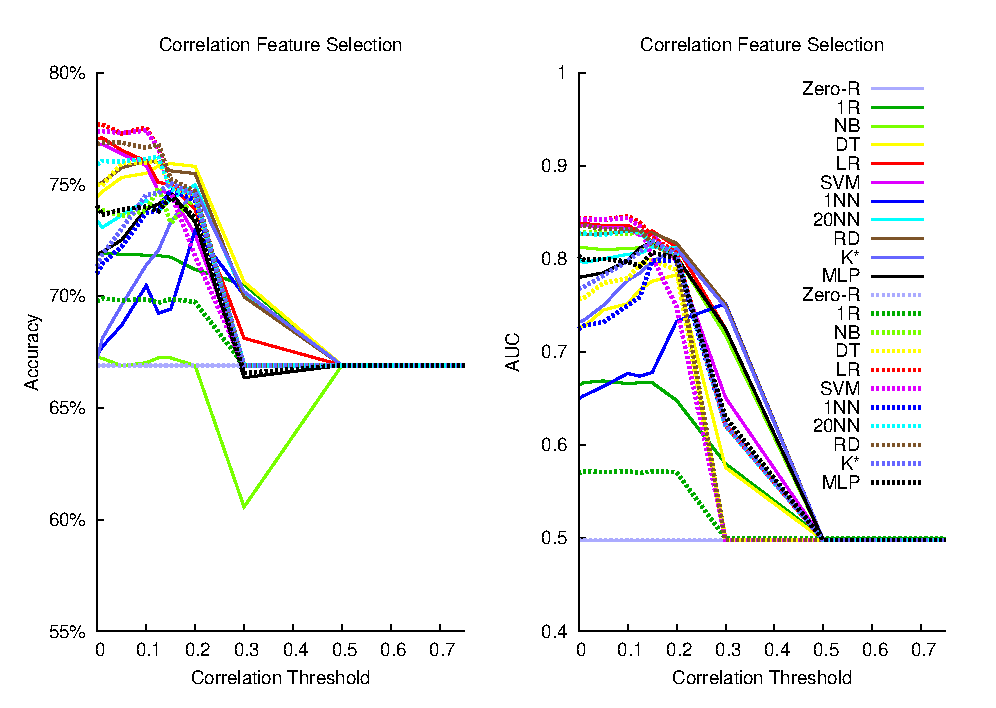
\includegraphics[width=\textwidth]{images/results/tr-corr.eps}
\caption{}
\label{fig:tr-threshold-corr}
\end{subfigure}
\caption{Comparison of accuracy and AUC between classifiers for feature selectors that discard features based on a threshold. Solid lines correspond to a result without discretisation, and dashed lines correspond to a result with discretisation.}
\label{fig:tr-threshold}
\end{figure}

\begin{figure}[htbp]
\ContinuedFloat
\begin{subfigure}{\textwidth}
\includegraphics[width=\textwidth]{images/results/tr-ig.eps}
\caption{}
\label{fig:tr-threshold-ig}
\end{subfigure}

\begin{subfigure}{\textwidth}
\includegraphics[width=\textwidth]{images/results/tr-oner.eps}
\caption{}
\label{fig:tr-threshold-oner}
\end{subfigure}
\caption{Comparison of accuracy and AUC between classifiers for feature selectors that discard features based on a threshold. Solid lines correspond to a result without discretisation, and dashed lines correspond to a result with discretisation.}
\end{figure}



In terms of classification accuracy, we did not find a lot of variation
between all classifiers, with Zero-R producing 66.91\% accuracy and 77.81\%
being the best we achieved -- an improvement of just over 10\%. The AUC of
the 11 classifiers we tested ranged from 0.498 with Zero-R to 0.846 with
logistic regression. Logistic regression, the \textit{de facto} method
used in LOS classification, performed consistently better than the others
across all feature
selection methods, but only when the feature set was not heavily reduced by
the feature selector: in these cases, such as the results from Figure
\ref{fig:tr-nothreshold-cfs-acc} showing classifier performance with features
selected by CFS, C4.5 decision trees and nearest
neighbour methods have higher accuracy than logistic regression. This is also
apparent from the graphs in Figure \ref{fig:tr-threshold}: for all three
feature selection methods, as we increase the threshold, logistic regression
drops in performance after the initial few thresholds and is outperformed by
C4.5 and the various nearest neighbour classifiers ($k$-NN with 1 and 20
neighbours and K*), as well as our Ranked Distance algorithm.
This is true for both accuracy and AUC.

We found that in most cases, the SVM did not achieve a higher accuracy or
AUC than logistic regression with the same features even though SVMs are
considered the state-of-the-art in classification algorithms. Additionally,
as the feature set was reduced, the discriminating ability of SVMs (as
indicated by the AUC) decreased more than their accuracy: this is particularly
noticeable in Figure \ref{fig:tr-threshold-oner}, where the AUC of the SVM
drops sharply to below the AUC of even the 1R classifier at the 67.905\%
threshold, where there are
only 4 features. SVMs have not been used in a LOS classification problem like
ours, so there will need to be further work carried out in order to assess the
suitability of using SVMs to classify patient LOS.

Although the MLP has been investigated in studies attempting to identify
factors associated with longer LOS or mortality for trauma patients
\cite{Hunter2000,McGonigal1993}, leading to improved results with the neural
network, we did not see the MLP outperform all other classifiers with respect
to accuracy or AUC for any feature selection method for this data set. In fact,
the MLP often performed no better than any of the nearest neighbour
classifiers, which use a straightfoward mechanism of classifying unseen
examples. Even if the MLP had managed to achieve superior accuracy or AUC, the
``black box'' nature of its prediction decisions are a barrier for their
widespread use in medical decision-making.

Nearest neighbour approaches appear to have performed well on this data set in
both accuracy and AUC, especially in comparison to more sophisticated
classifiers and when the feature set is significantly reduced. From the graphs
in Figure \ref{fig:tr-threshold}, we can see that all the nearest neighbours
approaches perform similarly when the number of features is decreased, but our
Ranked Distance algorithm showed a statistically significant improvement over
other NN algorithms. This
improvement is not apparent at smaller feature sets, where using the standard
$k$-NN algorithm with 1 or 20 neighbours performs slightly better.
The performance of NN we observed in our results is
an interesting finding because nearest neighbours have not been commonly
applied in predicting the LOS, but there is intuitive appeal in the
case-by-case nature of how these algorithms classify new examples that should
be explored further. Unlike MLPs and SVMs, prediction decision of nearest
neighbours are more transparent and understandable. However, the major drawback
of NN algorithms is their storage requirement and the computational time
required to search for the nearest neighbours to make the classification.

There is a limitation to our findings that needs to be noted: we did not
attempt to tune the parameters of the classifiers in order to find the ones
that resulted in the best performance, so our statements are based on the
results of the default parameters of each classifier.
MLPs in particular are sensitive to
the network architecture, so it is likely that its accuracy and AUC could be
improved if the parameters were selected to optimise its performance on this
data set.

\subsection{General Hospital Data}
In Figures \ref{fig:pt-nothreshold} and \ref{fig:pt-threshold}, we compare the
performance of the classifiers we used on the general hospital data set. In
contrast to the trauma data, we were able to achieve very high accuracy and
AUC on this data set using the exact same classifiers and feature selection
methods. Instead of only a 10\% improvement from Zero-R by the best classifier
in the trauma data, we were able to achieve an accuracy of 98.23\%, which is
an increase of over 20\% from the Zero-R accuracy on this data set of 75.64\%.
Additionally, we also managed to observe very high ($>0.97$) AUC figures for
all classifiers except Zero-R and 1R.

\begin{figure}[htbp]
\begin{subfigure}{.48\textwidth}
\includegraphics[width=\textwidth]{images/results/pt-nofs-acc.eps}
\caption{}
\label{}
\end{subfigure}%
\begin{subfigure}{.55\textwidth}
\includegraphics[width=\textwidth]{images/results/pt-nofs-auc.eps}
\caption{}
\label{}
\end{subfigure}

\begin{subfigure}{.48\textwidth}
\includegraphics[width=\textwidth]{images/results/pt-cfs-acc.eps}
\caption{}
\label{}
\end{subfigure}%
\begin{subfigure}{.55\textwidth}
\includegraphics[width=\textwidth]{images/results/pt-cfs-auc.eps}
\caption{}
\label{}
\end{subfigure}

\begin{subfigure}{.48\textwidth}
\includegraphics[width=\textwidth]{images/results/pt-wrapper-acc.eps}
\caption{}
\label{}
\end{subfigure}%
\begin{subfigure}{.55\textwidth}
\includegraphics[width=\textwidth]{images/results/pt-wrapper-auc.eps}
\caption{}
\label{}
\end{subfigure}
\caption{Comparison of accuracy and AUC between classifiers for each non-threshold feature selection method, grouped by whether or not discretisation was applied.}
\label{fig:pt-nothreshold}
\end{figure}

\begin{figure}[htbp]
\begin{subfigure}{\textwidth}
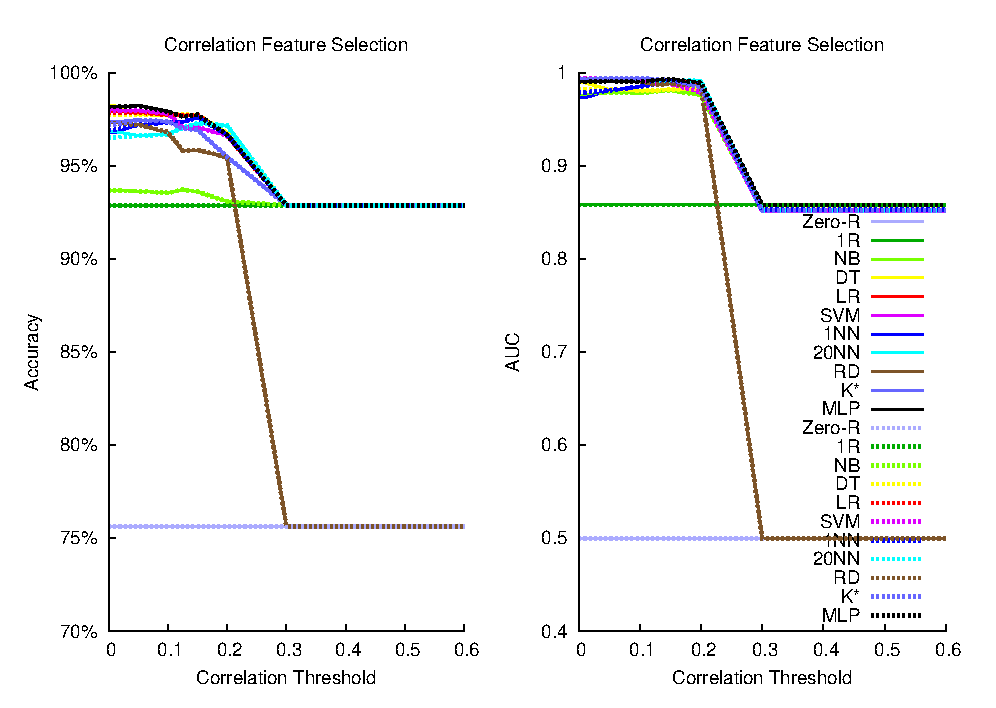
\includegraphics[width=\textwidth]{images/results/pt-corr.eps}
\caption{}
\label{fig:pt-threshold-corr}
\end{subfigure}
\ContinuedFloat
\begin{subfigure}{\textwidth}
\includegraphics[width=\textwidth]{images/results/pt-ig.eps}
\caption{}
\label{}
\end{subfigure}
\caption{Comparison of accuracy and AUC between classifiers for feature selectors that discard features based on a threshold. Solid lines correspond to a result without discretisation, and dashed lines correspond to a result with discretisation.}
\label{fig:pt-threshold}
\end{figure}

\begin{figure}[htbp]
\ContinuedFloat
\begin{subfigure}{\textwidth}
\includegraphics[width=\textwidth]{images/results/pt-oner.eps}
\caption{}
\label{}
\end{subfigure}
\caption[]{Comparison of accuracy and AUC between classifiers for feature selectors that discard features based on a threshold. Solid lines correspond to a result without discretisation, and dashed lines correspond to a result with discretisation.}
\end{figure}



Logistic regression and the SVM performed equal best in discriminating ability,
along with K* with an AUC of 0.994. We consider the performance of K* to be
superior because it was able to achieve this with 8 features out of 14, and
additionally it does not require any optimising of its parameters.
The AUC result of both logistic regression and the SVM were achieved with all
14 features. Although this is not a large number of features, simplifying the
inputs to a classifier is beneficial because it reduces the time needed for
training and classifying new examples. However, as indicated by the graphs in
Figure \ref{fig:pt-threshold} of AUC against threshold, and the bar charts in
Figure \ref{fig:pt-nothreshold}, the AUC of all classifiers except Zero-R and
1R was very close, around 0.98-0.99.

Notably, the MLP performed better than logistic regression on this data set
than on the trauma data, achieving better AUC with CFS and C4.5 wrapper feature
selection and better accuracy over all feature selection methods. This is a
surprising result as CFS and C4.5 wrapper select only 2 and 4 features
respectively. However, the major drawback of training the MLP with this data
set was the amount of time needed for one run of ten-fold cross-validation.
Even with only 14 features, the classifier required several hours to train.
Although we did not attempt to quantify the exact training time, it was by far
the slowest learning algorithm.
This is because the data set contained over 17000 training examples, which have
to be processed several times by the MLP until all of the weights between its
connections do not change more than a certain threshold.

Notice that in Figure \ref{fig:pt-threshold-corr}, both the accuracy and AUC
of Ranked Distance NN drop much more than for the other classifiers. This is at
a correlation coefficient threshold of 0.2, which reduces the feature set to
4 features. We noted in the discussion on classifiers for the trauma data set
that Ranked Distance NN performed worse for smaller feature sets than for larger
ones, and this is another example of this phenomenon. Recall that in Ranked
Distance NN, features are first ranked according to some similarity metric (we
have used the correlation coefficient), and then assigned a weight according
to their rank. The function we have used assigns rapidly decaying weights to
the features, which results in greater importance being placed on a few of
the features with the highest rank. Further work needs to be carried out to
investigate the cause of the poor performance on smaller feature sets, but
it is not altogether surprising: Ranked Distance NN performs best by using the
weighted distance contributions of all features, and by significantly reducing
their number we can expect to sharply reduce its ability to differentiate
between neighbours. There is also scope for investigating other weight
assignment functions which would work better in reduced-feature situations.

\section{Effect of Discretisation}
We touched briefly upon the effect of discretisation on the performance of the
classifiers used, but we would like to point out a few other things not
mentioned earlier. Firstly,
although discretisation improved the best accuracy and AUC for many
classifiers trained on the trauma data, this was only when using a larger
proportion of features: note the dotted lines in
Figures \ref{fig:tr-threshold-corr}, \ref{fig:tr-threshold-ig} and
\ref{fig:tr-threshold-oner} are above their solid line counterparts of the
same colour on the very left of the graph (where no features have been
discarded), but as we increase the threshold and more features are discarded,
the classifier using the discretised data set does not always perform better.
Notably, discretisation improves the accuracy and AUC of nearest neighbour
classifiers when few features have been removed, but as the number of features
decreases, these approaches perform worse with discretised features.

Although the results from discretisation with varying thresholds of the
correlation, information gain and 1R feature selectors are mixed, the graphs
in Figure \ref{fig:tr-nothreshold} show improvements in AUC and accuracy for
most classifiers in most of the situations, and show that discretisation is a
viable pre-processing technique for data mining problem. This improvement is
not present in the general hospital data set due to the nature of the data set:
as mentioned earlier, only one feature is discretised, which transforms it into
a single value. This single value does not help the classifier distinguish
between classes, and hence degrades performance.

Discretisation consistently improved the accuracy and AUC of the Na\"{i}ve
Bayes classifier, which suggests that it is more suitable for the data than the
classifier's assumption that continuous-valued features follow a normal
distribution.

Supervised discretisation such as the one we have used is very specific to the
data set, so it is difficult to draw general conclusions that will apply to
other learning problems. However, we have not yet seen this technique being
used in LOS prediction problems, and we believe it is worth investigating
when approaching a new learning problem.

\section{Summary}
In this section we have presented and discussed the main findings of our
work, examining the overall picture, and then detailing comparisons between
classifiers and feature selection methods in detail before concluding with a
few remarks on discretisation.

We found that irrespective of discretisation or feature selection, logistic
regression still performed better than other learning algorithms, which
reaffirms its use as the \textit{de facto} classifier in predictive medicine.
However, we were also able to achieve results that were almost as good using
nearest neighbour approaches combined with feature selection techniques,
neither of which have been investigated thoroughly in previous work. Our
proposed Ranked Distance algorithm was able to improve upon the accuracy and AUC of
the standard $k$-NN algorithm with the same number of neighbours, but we found
that its performance suffered when used in conjunction with feature selection.

In both the trauma and general hospital data sets, we were not able to
consistently improve the accuracy and AUC of all
classifiers with feature selection but we were able to sacrifice some
predictive power in order to use a drastically reduced feature set: for trauma
we found that K* with 11 features selected by a C4.5 wrapper performed only
slightly worse in discriminating between the two LOS classes than logistic
regression using 29 features, and for the hospital-wide data we achieved
0.983 AUC using only 2 features out of 14 using the MLP, 0.011 less than the
best result from logistic regression which required all 14 features. It is
therefore important to consider the trade-off between predictive ability,
speed and ease of understanding when making judgements about classifiers.

Finally, we pointed out that although discretisation was able to improve
classifier performance, this effect was less noticeable when more features
were discarded from feature selection. Discretisation has not been used
extensively in the LOS prediction literature, so our work will serve as a
starting point for further investigation.
